\section{Luồng quản lý intent/entity/response/rule/story/action}

Luồng này mô tả nhóm thao tác quản trị cấu hình tri thức hội thoại của chatbot, bao gồm intent, entity, response, rule, story và action. Đây là luồng quản lý cốt lõi để duy trì khả năng hiểu câu hỏi, tổ chức phản hồi và kiểm soát logic hội thoại của Rasa theo thời gian.

\begin{figure}[H]
    \centering
    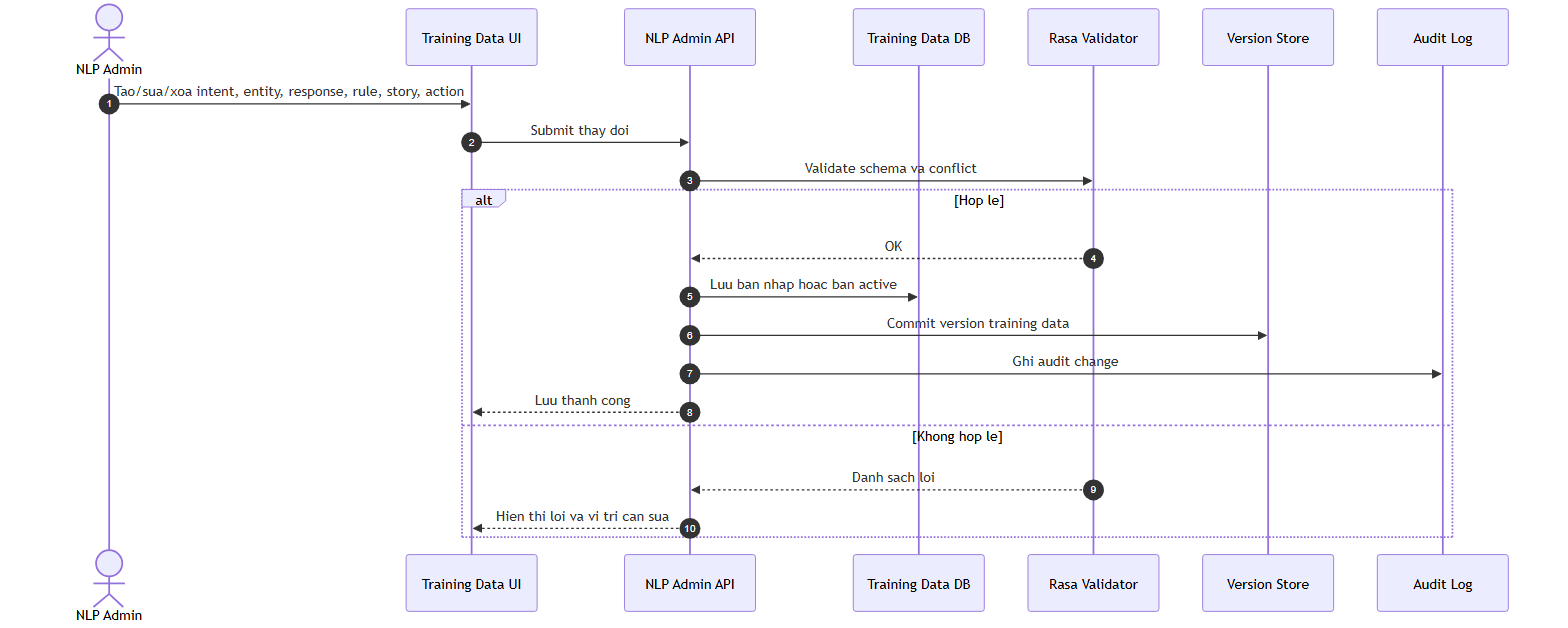
\includegraphics[width=\textwidth]{content/source/mermaid_sequence/seq_05.png}
    \caption{Luồng quản lý intent/entity/response/rule/story/action}
\end{figure}

Theo sequence, người quản trị tạo mới, cập nhật hoặc xóa các phần tử hội thoại trên giao diện; dữ liệu được gửi tới backend quản trị thông qua các API riêng cho từng loại đối tượng; backend xác thực, lưu trữ, rồi đồng bộ trở lại trạng thái mới cho frontend. Luồng này không chỉ phục vụ việc nhập dữ liệu NLU mà còn là cơ sở để tạo rule, story và response phục vụ suy diễn hội thoại trong Rasa.
